\documentclass[10pt]{article} % For LaTeX2e
\usepackage[preprint]{tmlr-template/tmlr}
% If accepted, instead use the following line for the camera-ready submission:
%\usepackage[accepted]{tmlr}
% To de-anonymize and remove mentions to TMLR (for example for posting to preprint servers), instead use the following:
% \usepackage[preprint]{tmlr}

%%%%% NEW MATH DEFINITIONS %%%%%

\usepackage{amsmath,amsfonts,bm}

% Mark sections of captions for referring to divisions of figures
\newcommand{\figleft}{{\em (Left)}}
\newcommand{\figcenter}{{\em (Center)}}
\newcommand{\figright}{{\em (Right)}}
\newcommand{\figtop}{{\em (Top)}}
\newcommand{\figbottom}{{\em (Bottom)}}
\newcommand{\captiona}{{\em (a)}}
\newcommand{\captionb}{{\em (b)}}
\newcommand{\captionc}{{\em (c)}}
\newcommand{\captiond}{{\em (d)}}

% Highlight a newly defined term
\newcommand{\newterm}[1]{{\bf #1}}


% Figure reference, lower-case.
\def\figref#1{figure~\ref{#1}}
% Figure reference, capital. For start of sentence
\def\Figref#1{Figure~\ref{#1}}
\def\twofigref#1#2{figures \ref{#1} and \ref{#2}}
\def\quadfigref#1#2#3#4{figures \ref{#1}, \ref{#2}, \ref{#3} and \ref{#4}}
% Section reference, lower-case.
\def\secref#1{section~\ref{#1}}
% Section reference, capital.
\def\Secref#1{Section~\ref{#1}}
% Reference to two sections.
\def\twosecrefs#1#2{sections \ref{#1} and \ref{#2}}
% Reference to three sections.
\def\secrefs#1#2#3{sections \ref{#1}, \ref{#2} and \ref{#3}}
% Reference to an equation, lower-case.
\def\eqref#1{equation~\ref{#1}}
% Reference to an equation, upper case
\def\Eqref#1{Equation~\ref{#1}}
% A raw reference to an equation---avoid using if possible
\def\plaineqref#1{\ref{#1}}
% Reference to a chapter, lower-case.
\def\chapref#1{chapter~\ref{#1}}
% Reference to an equation, upper case.
\def\Chapref#1{Chapter~\ref{#1}}
% Reference to a range of chapters
\def\rangechapref#1#2{chapters\ref{#1}--\ref{#2}}
% Reference to an algorithm, lower-case.
\def\algref#1{algorithm~\ref{#1}}
% Reference to an algorithm, upper case.
\def\Algref#1{Algorithm~\ref{#1}}
\def\twoalgref#1#2{algorithms \ref{#1} and \ref{#2}}
\def\Twoalgref#1#2{Algorithms \ref{#1} and \ref{#2}}
% Reference to a part, lower case
\def\partref#1{part~\ref{#1}}
% Reference to a part, upper case
\def\Partref#1{Part~\ref{#1}}
\def\twopartref#1#2{parts \ref{#1} and \ref{#2}}

\def\ceil#1{\lceil #1 \rceil}
\def\floor#1{\lfloor #1 \rfloor}
\def\1{\bm{1}}
\newcommand{\train}{\mathcal{D}}
\newcommand{\valid}{\mathcal{D_{\mathrm{valid}}}}
\newcommand{\test}{\mathcal{D_{\mathrm{test}}}}

\def\eps{{\epsilon}}


% Random variables
\def\reta{{\textnormal{$\eta$}}}
\def\ra{{\textnormal{a}}}
\def\rb{{\textnormal{b}}}
\def\rc{{\textnormal{c}}}
\def\rd{{\textnormal{d}}}
\def\re{{\textnormal{e}}}
\def\rf{{\textnormal{f}}}
\def\rg{{\textnormal{g}}}
\def\rh{{\textnormal{h}}}
\def\ri{{\textnormal{i}}}
\def\rj{{\textnormal{j}}}
\def\rk{{\textnormal{k}}}
\def\rl{{\textnormal{l}}}
% rm is already a command, just don't name any random variables m
\def\rn{{\textnormal{n}}}
\def\ro{{\textnormal{o}}}
\def\rp{{\textnormal{p}}}
\def\rq{{\textnormal{q}}}
\def\rr{{\textnormal{r}}}
\def\rs{{\textnormal{s}}}
\def\rt{{\textnormal{t}}}
\def\ru{{\textnormal{u}}}
\def\rv{{\textnormal{v}}}
\def\rw{{\textnormal{w}}}
\def\rx{{\textnormal{x}}}
\def\ry{{\textnormal{y}}}
\def\rz{{\textnormal{z}}}

% Random vectors
\def\rvepsilon{{\mathbf{\epsilon}}}
\def\rvtheta{{\mathbf{\theta}}}
\def\rva{{\mathbf{a}}}
\def\rvb{{\mathbf{b}}}
\def\rvc{{\mathbf{c}}}
\def\rvd{{\mathbf{d}}}
\def\rve{{\mathbf{e}}}
\def\rvf{{\mathbf{f}}}
\def\rvg{{\mathbf{g}}}
\def\rvh{{\mathbf{h}}}
\def\rvu{{\mathbf{i}}}
\def\rvj{{\mathbf{j}}}
\def\rvk{{\mathbf{k}}}
\def\rvl{{\mathbf{l}}}
\def\rvm{{\mathbf{m}}}
\def\rvn{{\mathbf{n}}}
\def\rvo{{\mathbf{o}}}
\def\rvp{{\mathbf{p}}}
\def\rvq{{\mathbf{q}}}
\def\rvr{{\mathbf{r}}}
\def\rvs{{\mathbf{s}}}
\def\rvt{{\mathbf{t}}}
\def\rvu{{\mathbf{u}}}
\def\rvv{{\mathbf{v}}}
\def\rvw{{\mathbf{w}}}
\def\rvx{{\mathbf{x}}}
\def\rvy{{\mathbf{y}}}
\def\rvz{{\mathbf{z}}}

% Elements of random vectors
\def\erva{{\textnormal{a}}}
\def\ervb{{\textnormal{b}}}
\def\ervc{{\textnormal{c}}}
\def\ervd{{\textnormal{d}}}
\def\erve{{\textnormal{e}}}
\def\ervf{{\textnormal{f}}}
\def\ervg{{\textnormal{g}}}
\def\ervh{{\textnormal{h}}}
\def\ervi{{\textnormal{i}}}
\def\ervj{{\textnormal{j}}}
\def\ervk{{\textnormal{k}}}
\def\ervl{{\textnormal{l}}}
\def\ervm{{\textnormal{m}}}
\def\ervn{{\textnormal{n}}}
\def\ervo{{\textnormal{o}}}
\def\ervp{{\textnormal{p}}}
\def\ervq{{\textnormal{q}}}
\def\ervr{{\textnormal{r}}}
\def\ervs{{\textnormal{s}}}
\def\ervt{{\textnormal{t}}}
\def\ervu{{\textnormal{u}}}
\def\ervv{{\textnormal{v}}}
\def\ervw{{\textnormal{w}}}
\def\ervx{{\textnormal{x}}}
\def\ervy{{\textnormal{y}}}
\def\ervz{{\textnormal{z}}}

% Random matrices
\def\rmA{{\mathbf{A}}}
\def\rmB{{\mathbf{B}}}
\def\rmC{{\mathbf{C}}}
\def\rmD{{\mathbf{D}}}
\def\rmE{{\mathbf{E}}}
\def\rmF{{\mathbf{F}}}
\def\rmG{{\mathbf{G}}}
\def\rmH{{\mathbf{H}}}
\def\rmI{{\mathbf{I}}}
\def\rmJ{{\mathbf{J}}}
\def\rmK{{\mathbf{K}}}
\def\rmL{{\mathbf{L}}}
\def\rmM{{\mathbf{M}}}
\def\rmN{{\mathbf{N}}}
\def\rmO{{\mathbf{O}}}
\def\rmP{{\mathbf{P}}}
\def\rmQ{{\mathbf{Q}}}
\def\rmR{{\mathbf{R}}}
\def\rmS{{\mathbf{S}}}
\def\rmT{{\mathbf{T}}}
\def\rmU{{\mathbf{U}}}
\def\rmV{{\mathbf{V}}}
\def\rmW{{\mathbf{W}}}
\def\rmX{{\mathbf{X}}}
\def\rmY{{\mathbf{Y}}}
\def\rmZ{{\mathbf{Z}}}

% Elements of random matrices
\def\ermA{{\textnormal{A}}}
\def\ermB{{\textnormal{B}}}
\def\ermC{{\textnormal{C}}}
\def\ermD{{\textnormal{D}}}
\def\ermE{{\textnormal{E}}}
\def\ermF{{\textnormal{F}}}
\def\ermG{{\textnormal{G}}}
\def\ermH{{\textnormal{H}}}
\def\ermI{{\textnormal{I}}}
\def\ermJ{{\textnormal{J}}}
\def\ermK{{\textnormal{K}}}
\def\ermL{{\textnormal{L}}}
\def\ermM{{\textnormal{M}}}
\def\ermN{{\textnormal{N}}}
\def\ermO{{\textnormal{O}}}
\def\ermP{{\textnormal{P}}}
\def\ermQ{{\textnormal{Q}}}
\def\ermR{{\textnormal{R}}}
\def\ermS{{\textnormal{S}}}
\def\ermT{{\textnormal{T}}}
\def\ermU{{\textnormal{U}}}
\def\ermV{{\textnormal{V}}}
\def\ermW{{\textnormal{W}}}
\def\ermX{{\textnormal{X}}}
\def\ermY{{\textnormal{Y}}}
\def\ermZ{{\textnormal{Z}}}

% Vectors
\def\vzero{{\bm{0}}}
\def\vone{{\bm{1}}}
\def\vmu{{\bm{\mu}}}
\def\vtheta{{\bm{\theta}}}
\def\va{{\bm{a}}}
\def\vb{{\bm{b}}}
\def\vc{{\bm{c}}}
\def\vd{{\bm{d}}}
\def\ve{{\bm{e}}}
\def\vf{{\bm{f}}}
\def\vg{{\bm{g}}}
\def\vh{{\bm{h}}}
\def\vi{{\bm{i}}}
\def\vj{{\bm{j}}}
\def\vk{{\bm{k}}}
\def\vl{{\bm{l}}}
\def\vm{{\bm{m}}}
\def\vn{{\bm{n}}}
\def\vo{{\bm{o}}}
\def\vp{{\bm{p}}}
\def\vq{{\bm{q}}}
\def\vr{{\bm{r}}}
\def\vs{{\bm{s}}}
\def\vt{{\bm{t}}}
\def\vu{{\bm{u}}}
\def\vv{{\bm{v}}}
\def\vw{{\bm{w}}}
\def\vx{{\bm{x}}}
\def\vy{{\bm{y}}}
\def\vz{{\bm{z}}}


% Elements of vectors
\def\evalpha{{\alpha}}
\def\evbeta{{\beta}}
\def\evepsilon{{\epsilon}}
\def\evlambda{{\lambda}}
\def\evomega{{\omega}}
\def\evmu{{\mu}}
\def\evpsi{{\psi}}
\def\evsigma{{\sigma}}
\def\evtheta{{\theta}}
\def\eva{{a}}
\def\evb{{b}}
\def\evc{{c}}
\def\evd{{d}}
\def\eve{{e}}
\def\evf{{f}}
\def\evg{{g}}
\def\evh{{h}}
\def\evi{{i}}
\def\evj{{j}}
\def\evk{{k}}
\def\evl{{l}}
\def\evm{{m}}
\def\evn{{n}}
\def\evo{{o}}
\def\evp{{p}}
\def\evq{{q}}
\def\evr{{r}}
\def\evs{{s}}
\def\evt{{t}}
\def\evu{{u}}
\def\evv{{v}}
\def\evw{{w}}
\def\evx{{x}}
\def\evy{{y}}
\def\evz{{z}}

% Matrix
\def\mA{{\bm{A}}}
\def\mB{{\bm{B}}}
\def\mC{{\bm{C}}}
\def\mD{{\bm{D}}}
\def\mE{{\bm{E}}}
\def\mF{{\bm{F}}}
\def\mG{{\bm{G}}}
\def\mH{{\bm{H}}}
\def\mI{{\bm{I}}}
\def\mJ{{\bm{J}}}
\def\mK{{\bm{K}}}
\def\mL{{\bm{L}}}
\def\mM{{\bm{M}}}
\def\mN{{\bm{N}}}
\def\mO{{\bm{O}}}
\def\mP{{\bm{P}}}
\def\mQ{{\bm{Q}}}
\def\mR{{\bm{R}}}
\def\mS{{\bm{S}}}
\def\mT{{\bm{T}}}
\def\mU{{\bm{U}}}
\def\mV{{\bm{V}}}
\def\mW{{\bm{W}}}
\def\mX{{\bm{X}}}
\def\mY{{\bm{Y}}}
\def\mZ{{\bm{Z}}}
\def\mBeta{{\bm{\beta}}}
\def\mPhi{{\bm{\Phi}}}
\def\mLambda{{\bm{\Lambda}}}
\def\mSigma{{\bm{\Sigma}}}

% Tensor
\DeclareMathAlphabet{\mathsfit}{\encodingdefault}{\sfdefault}{m}{sl}
\SetMathAlphabet{\mathsfit}{bold}{\encodingdefault}{\sfdefault}{bx}{n}
\newcommand{\tens}[1]{\bm{\mathsfit{#1}}}
\def\tA{{\tens{A}}}
\def\tB{{\tens{B}}}
\def\tC{{\tens{C}}}
\def\tD{{\tens{D}}}
\def\tE{{\tens{E}}}
\def\tF{{\tens{F}}}
\def\tG{{\tens{G}}}
\def\tH{{\tens{H}}}
\def\tI{{\tens{I}}}
\def\tJ{{\tens{J}}}
\def\tK{{\tens{K}}}
\def\tL{{\tens{L}}}
\def\tM{{\tens{M}}}
\def\tN{{\tens{N}}}
\def\tO{{\tens{O}}}
\def\tP{{\tens{P}}}
\def\tQ{{\tens{Q}}}
\def\tR{{\tens{R}}}
\def\tS{{\tens{S}}}
\def\tT{{\tens{T}}}
\def\tU{{\tens{U}}}
\def\tV{{\tens{V}}}
\def\tW{{\tens{W}}}
\def\tX{{\tens{X}}}
\def\tY{{\tens{Y}}}
\def\tZ{{\tens{Z}}}


% Graph
\def\gA{{\mathcal{A}}}
\def\gB{{\mathcal{B}}}
\def\gC{{\mathcal{C}}}
\def\gD{{\mathcal{D}}}
\def\gE{{\mathcal{E}}}
\def\gF{{\mathcal{F}}}
\def\gG{{\mathcal{G}}}
\def\gH{{\mathcal{H}}}
\def\gI{{\mathcal{I}}}
\def\gJ{{\mathcal{J}}}
\def\gK{{\mathcal{K}}}
\def\gL{{\mathcal{L}}}
\def\gM{{\mathcal{M}}}
\def\gN{{\mathcal{N}}}
\def\gO{{\mathcal{O}}}
\def\gP{{\mathcal{P}}}
\def\gQ{{\mathcal{Q}}}
\def\gR{{\mathcal{R}}}
\def\gS{{\mathcal{S}}}
\def\gT{{\mathcal{T}}}
\def\gU{{\mathcal{U}}}
\def\gV{{\mathcal{V}}}
\def\gW{{\mathcal{W}}}
\def\gX{{\mathcal{X}}}
\def\gY{{\mathcal{Y}}}
\def\gZ{{\mathcal{Z}}}

% Sets
\def\sA{{\mathbb{A}}}
\def\sB{{\mathbb{B}}}
\def\sC{{\mathbb{C}}}
\def\sD{{\mathbb{D}}}
% Don't use a set called E, because this would be the same as our symbol
% for expectation.
\def\sF{{\mathbb{F}}}
\def\sG{{\mathbb{G}}}
\def\sH{{\mathbb{H}}}
\def\sI{{\mathbb{I}}}
\def\sJ{{\mathbb{J}}}
\def\sK{{\mathbb{K}}}
\def\sL{{\mathbb{L}}}
\def\sM{{\mathbb{M}}}
\def\sN{{\mathbb{N}}}
\def\sO{{\mathbb{O}}}
\def\sP{{\mathbb{P}}}
\def\sQ{{\mathbb{Q}}}
\def\sR{{\mathbb{R}}}
\def\sS{{\mathbb{S}}}
\def\sT{{\mathbb{T}}}
\def\sU{{\mathbb{U}}}
\def\sV{{\mathbb{V}}}
\def\sW{{\mathbb{W}}}
\def\sX{{\mathbb{X}}}
\def\sY{{\mathbb{Y}}}
\def\sZ{{\mathbb{Z}}}

% Entries of a matrix
\def\emLambda{{\Lambda}}
\def\emA{{A}}
\def\emB{{B}}
\def\emC{{C}}
\def\emD{{D}}
\def\emE{{E}}
\def\emF{{F}}
\def\emG{{G}}
\def\emH{{H}}
\def\emI{{I}}
\def\emJ{{J}}
\def\emK{{K}}
\def\emL{{L}}
\def\emM{{M}}
\def\emN{{N}}
\def\emO{{O}}
\def\emP{{P}}
\def\emQ{{Q}}
\def\emR{{R}}
\def\emS{{S}}
\def\emT{{T}}
\def\emU{{U}}
\def\emV{{V}}
\def\emW{{W}}
\def\emX{{X}}
\def\emY{{Y}}
\def\emZ{{Z}}
\def\emSigma{{\Sigma}}

% entries of a tensor
% Same font as tensor, without \bm wrapper
\newcommand{\etens}[1]{\mathsfit{#1}}
\def\etLambda{{\etens{\Lambda}}}
\def\etA{{\etens{A}}}
\def\etB{{\etens{B}}}
\def\etC{{\etens{C}}}
\def\etD{{\etens{D}}}
\def\etE{{\etens{E}}}
\def\etF{{\etens{F}}}
\def\etG{{\etens{G}}}
\def\etH{{\etens{H}}}
\def\etI{{\etens{I}}}
\def\etJ{{\etens{J}}}
\def\etK{{\etens{K}}}
\def\etL{{\etens{L}}}
\def\etM{{\etens{M}}}
\def\etN{{\etens{N}}}
\def\etO{{\etens{O}}}
\def\etP{{\etens{P}}}
\def\etQ{{\etens{Q}}}
\def\etR{{\etens{R}}}
\def\etS{{\etens{S}}}
\def\etT{{\etens{T}}}
\def\etU{{\etens{U}}}
\def\etV{{\etens{V}}}
\def\etW{{\etens{W}}}
\def\etX{{\etens{X}}}
\def\etY{{\etens{Y}}}
\def\etZ{{\etens{Z}}}

% The true underlying data generating distribution
\newcommand{\pdata}{p_{\rm{data}}}
% The empirical distribution defined by the training set
\newcommand{\ptrain}{\hat{p}_{\rm{data}}}
\newcommand{\Ptrain}{\hat{P}_{\rm{data}}}
% The model distribution
\newcommand{\pmodel}{p_{\rm{model}}}
\newcommand{\Pmodel}{P_{\rm{model}}}
\newcommand{\ptildemodel}{\tilde{p}_{\rm{model}}}
% Stochastic autoencoder distributions
\newcommand{\pencode}{p_{\rm{encoder}}}
\newcommand{\pdecode}{p_{\rm{decoder}}}
\newcommand{\precons}{p_{\rm{reconstruct}}}

\newcommand{\laplace}{\mathrm{Laplace}} % Laplace distribution

\newcommand{\E}{\mathbb{E}}
\newcommand{\Ls}{\mathcal{L}}
\newcommand{\R}{\mathbb{R}}
\newcommand{\emp}{\tilde{p}}
\newcommand{\lr}{\alpha}
\newcommand{\reg}{\lambda}
\newcommand{\rect}{\mathrm{rectifier}}
\newcommand{\softmax}{\mathrm{softmax}}
\newcommand{\sigmoid}{\sigma}
\newcommand{\softplus}{\zeta}
\newcommand{\KL}{D_{\mathrm{KL}}}
\newcommand{\Var}{\mathrm{Var}}
\newcommand{\standarderror}{\mathrm{SE}}
\newcommand{\Cov}{\mathrm{Cov}}
% Wolfram Mathworld says $L^2$ is for function spaces and $\ell^2$ is for vectors
% But then they seem to use $L^2$ for vectors throughout the site, and so does
% wikipedia.
\newcommand{\normlzero}{L^0}
\newcommand{\normlone}{L^1}
\newcommand{\normltwo}{L^2}
\newcommand{\normlp}{L^p}
\newcommand{\normmax}{L^\infty}

\newcommand{\parents}{Pa} % See usage in notation.tex. Chosen to match Daphne's book.

\DeclareMathOperator*{\argmax}{arg\,max}
\DeclareMathOperator*{\argmin}{arg\,min}

\DeclareMathOperator{\sign}{sign}
\DeclareMathOperator{\Tr}{Tr}
\let\ab\allowbreak


\usepackage{hyperref}
\usepackage{url}
\usepackage{graphicx}
\usepackage{amsmath}
\usepackage{amssymb}
\usepackage{bm}
\usepackage{mathtools}
\usepackage[OT1]{fontenc}

\def\vTheta{{\bm{\Theta}}}
\def\vPhi{{\bm{\Phi}}}
\newcommand{\trainloss}{\mathcal{L}_{\sS}}
\newcommand{\batchloss}{\mathcal{L}_{\sB}}
\newcommand{\genloss}{\mathcal{L}_{\sQ}}

\DeclareRobustCommand{\titlevq}{\bm{q}}

\title{Double Descent 2: Feature learning and Frozen kernel Model-Wise Double Descents}

% Anonymous submission
\author{\name Viktor Vesel\'{y} \email v.vesely@student.rug.nl \\
\addr University of Groningen
} 

\newcommand{\fix}{\marginpar{FIX}}
\newcommand{\new}{\marginpar{NEW}}

\def\month{MM}
\def\year{YYYY}
\def\openreview{\url{https://openreview.net/forum?id=XXXX}}

\begin{document}

\maketitle

\begin{abstract}
    Double descent describes the non-monotonic generalization behavior of neural networks as model capacity or training time increases. In this work, we identify two distinct mechanisms underlying model-wise double descent: feature-learning double descent (FLDD) and frozen-kernel double descent (FKDD). We show that FLDD arises when neural networks learn features that accelerate the fitting of noisy training labels, leading to a transient deterioration in generalization. In contrast, FKDD emerges from the slow fitting of residual errors along small-eigenvalue modes of the empirical neural tangent kernel, which transfer poorly to unseen data. We distinguish these mechanisms through controlled comparisons between feature-learning and frozen-kernel dynamics and introduce a sample-level measure of how feature learning facilitates noise fitting. Through targeted feature-learning ablations, we identify training samples responsible for forming noise-fitting features and demonstrate that suppressing their contribution to feature learning reduces the early double-descent peak without preventing the model from fitting those samples.
\end{abstract}

\section{Introduction}

\begin{figure}[h]
    \centering
    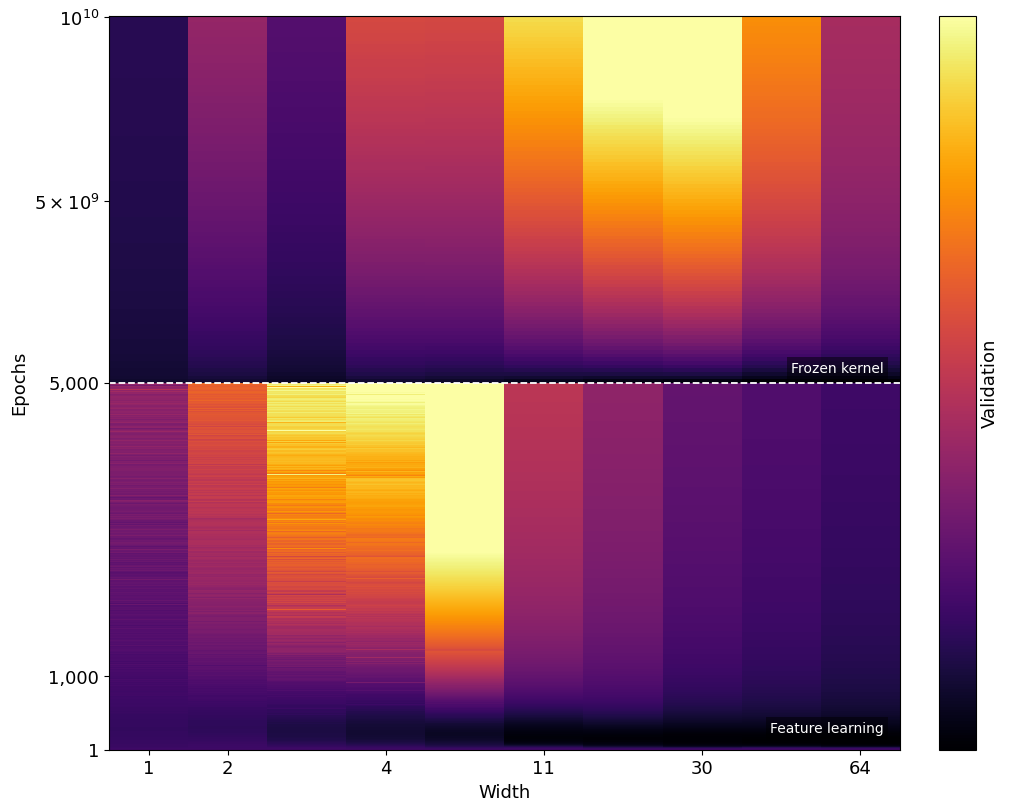
\includegraphics[width=0.9\columnwidth]{../showcase_of_double_dd.png}
    \caption{Showcase of two distinct model-wise double descents happening at a different place for the same task, architecture, data ordering, learning rates, amount of learnable parameters. The lower part of the plot shows the early Feature Learning double descent, the upper part of the plot shows the later frozen kernel double descent. Two distinct mechanims give rise to each, see the text for full explanation.}
    \label{fig:double-dd-showcase}
\end{figure}

\subsection{Contributions}

Focusing on MNIST and CIFAR10.

\begin{itemize}
    \item \textbf{(C1) There are two double descents} We identify for each deep architecture and a task there are two double desents. One that happens sooner (epochs and widths) due to feature learning accelerating the learning of a noise. Second happening much later (with epochs) that happens much later due to slow learning modes (define by the smallest non-zero eigenvalue of the empirical ntk) producing large parameters and transfering badly on validaiton. 

    \item \textbf{(C2) Identification of feature learning double descent mechanism} We propose and test a mechanism for the rise of the feature learning double descent to be a formation of features which aid with learning noise. We identify samples that cause these features to form and disable feature learning for them (but the model is still being able to fit them) we observe a significant drop on the double desent peak. 

\end{itemize}

\section{Background}

We consider a supervised learning setting with a training dataset $\sS = \{\vx_s, \vy_s\}_{l=1}^{S}$ of $S$ i.i.d.\ samples, where $\vx \in \sR^{d_x}$ denotes the input and $\vy \in \sR^{d_y}$ the corresponding real valued output for regression and $\vy \in \{0, 1\}^{d_y}$ the one-hot vector over $d_y$ classes for classification. Analogously, $\sQ = \{\vx_q, \vy_q\}_{q=1}^{Q}$ defines the testing dataset with $Q$ samples.

We define $\vtheta_{n,p} \in \sR^{p}$ to be $p$ parameters of a neural network $f_{\vtheta}$ trained for $n$ epochs. We train the parameters by minimizing the training loss $\mathcal{L}_{\sS}$ which is instantiated to MSE for regression tasks and CE for classification tasks. Test loss $\mathcal{L}_{\sQ}$ is used to measure the final performance.

We train our models with the plain stochastic gradient descent for random batches $\sB \subset \sS$ and a constant learning rate $\eta$, yielding the update rule $\theta_{t + 1} = \theta{t} + \eta \nabla_{\theta_t} \batchloss(\theta_t)$.

To induce double descent in classification tasks, we introduce label noise at a rate $\eta \in [0,1]$. Before training, we select a fraction $\eta$ of the training samples uniformly at random and replace each selected label with a label drawn uniformly from the remaining $d_y - 1$ classes for classification or drawn uniformly from other samples otputs for regression. Both the selected samples and their corrupted labels remain fixed throughout training, while the test labels remain unchanged.

\subsection{Taylor approximation of the SGD learning dynamics}


\paragraph{Definitions} We follow the standard calculus notation for stochastic gradient descent on a training batch  $\sB \subset \sS$ 

\begin{align*}
    \vb \coloneqq (f_\vtheta(\vx_0): \ldots : f_\vtheta(\vx_{|\sB|})), \quad \vx_i \in \sB  \quad & \text{Batch outputs' concatenation;} \\
    \vg_\sB \coloneqq \nabla_\vb \batchloss \quad & \text{Output training gradient;}\\
    \mJ_{\sB} \coloneqq \nabla_\theta \vb \quad &  \text{Jacobian of batch otuputs;}\\
    \vp_\sB \coloneqq  \mJ^\top_{\sB} \vg_\sB  \quad & \text{Parameter training gradient for the batch.}\\
    K_{\sX \sY} \coloneqq  \mJ_{\sX} \mJ^\top_{\sY}  \quad & \text{Cross-kernel matrix between set $\sX$ and set $\sY$}
\end{align*}


\paragraph{Feature learning identifications} We work with the following second taylor approximation of the traing loss change $\Delta \trainloss$ for the actual SGD step
\begin{align}
    \Delta \trainloss &= \sum_{\sB \subset \sS} \Delta \batchloss \\
    \Delta \batchloss &\approx \Delta t \dot{\batchloss} + \frac{(\Delta t)^2}{2} \ddot{\batchloss} \label{eq:taylor-approx} \\
    \dot{\batchloss} &= -\vg^\top_\sB \mJ_{\sB} \mJ^\top_{\sB} \vg_\sB \\
    \ddot{\batchloss} &= \underbrace{\vp_\sB^\top \mJ^\top_\sB (\nabla^2_f \trainloss) \vp_\sB }_{\text{Loss curvature}} + \underbrace{\vp_\sB^\top \left( \sum^{d_x}_{i} (\vg_\sB)_i (\nabla^2_\vtheta f)_i \right) \vp_\sB }_{\text{Feature-learning curvature}}
\end{align}
with the time step being equal to the learning rate $\Delta t = \eta$. However, later we show that the approximation in Equation~\ref{eq:taylor-approx} is not numerically sufficient due to the loss changing non-linearly across the fixed path of the SGD update, more on that in Appendix~\ref{ap:taylor-integrated}. The derivation of the terms is included in Appendix~\ref{ap:taylor-derivation}. Second order taylor approximation is the minimal order sufficient to explicitly identify the feature learning effect. Notice that the feature leanring term is precisely 0 with the frozen kernel models which gives us a way to naturally define what feature learning is.

We follow a loose definition of feature learning, where the current task and architecture pair cause the Jacobian to substantially diverge from its initial value $\nabla_\vtheta f(\vtheta_0)$, the feature learning term can then be used to capture the instantenous effect of the change in the jacobian on the training/test loss. 

\paragraph{Transfer on the validation}

Equations for the first order transfer metric definition per sample


\subsection{Kernel regression}

Formalize the kernel regression quickly here and then just reuse it in the later sections

\section{Methodology}


\subsection{Identification of two Double Descent mechanisms}


\paragraph{Showing the distinction} We can identify the two distinct double double descents by starting from a common point: with the same architecture, task, data ordering, initial features, weight initializations, learning rate, epoch budget $T$ etc. Then we continue with an feature learning ablation, we train two copies of the same starting point one with feature feature learning where the parameters fully free to move and the second copy is with frozen kernel, where the initial features stay the same. The cleanest way of freezing the kernel for a function $f_{\vtheta_t}$ is to introduce a second parameter vector $\vw \in \sR^{\lvert \vtheta \rvert}$ which learns the tangent features:
\begin{equation} \label{eq:frozen-kernel}
    \bar{f}_{\vtheta_t} (\vx; \vw) = f_{\vtheta_t} (\vx) +  (\nabla_{\vtheta_t} f_{\vtheta_t}) \vw 
\end{equation}
where $\vtheta_t$ will be frozen and $\vw$ will be updated freely. Substituting $\vtheta_0$ and learning showcases that the double descent dissapears for the frozen kernel regime (show a figure here).

To 

\paragraph{Showing the coexistence} The coexistence of the two DDs for the same full feature learning run is this:
- for the tasks and architectures presented here it is computationally feasible to empirically observe the FKDD in the actual feature learning run since as seen from the figure the occurance of FKDD happens in very distant epochs (around $5 \cdot 10^{9}$)
- thus we based the coexistence of the two DDs based on the assumption that the movement of the kernel (feature learning) slows down as the training progresses (which is not theoratically guaranteed but it is a common empirical behavior \citep{atanasov2021neuralnetworkskernelleaners})
- Using this assumption we can freeze the actual learned model $\vtheta_T$ by again using Equation \ref{eq:frozen-kernel} and using kernel regression to display the validation error given the frozen kernel assumption

\subsection{Feature learning Double Descent Mechanism}

In frozen kernel regime the peak is caused by the following conditions: the empirical ntk contains small non-zero eigenvalues AND that eigmode has some residual power left (gradient wants to fit it) AND  that eigenmode transfers harmfully on the validation. The intuitve mechanism is then that in order to fit the small eigenmodes it requires large coefficients, which transfer very poorly on the validation (since they are taylord for the noise). The frozen kernel regime operates in the eigenmodes, our hypothesis about the FL DD operates from the samples' perspective. We call this double descent FKDD

We hypothesize that the Fl DD is caused by some training samples constructing features which make learning noise samples easier, conditions: i) there will be samples which create features which are beneficial for the noise AND ii) the network has sufficient capacity to fit the noise (and it will be fitted quickly) AND iii) the noise samples will transfer VERY poorly to the validation. We call this double descent FLDD.

Now formulating i) ii) and iii) exactly

i) comes from the following property. Let $\sL \subset \sB$ be the noise samples in the current training batch. We can measure how easily can the noise be learned under the current features/jacobian lets call this property $l(\vtheta)$:
\begin{align}
    l(\vtheta) &= \vg^\top_\sL J_\sL \vp_\sB \\
    \dot{l}(\vtheta) &=  \underbrace{\dot{\vg}^\top_\sL J_\sL \vp_\sB}_\text{Changes in the loss} + \underbrace{\vg^\top_\sL \dot{J}_\sL \vp_\sB}_\text{Changes in the features} + \underbrace{\vg^\top_\sL J_\sL \dot{\vp}_\sB}_\text{SGD does not change the direction in one step thus $0$}
\end{align}
we are only interested how much does the feature learning influence the ease of noise fitting (the middle term lets call it $h_i$) .


We are not claiming that these are the sufficient conditions for the FLDD to arise, we acknowledge its depedence also on other factors such as noise percentage, optimizers, batch size, and learning rate (citations here). We merely identify the feature learning contributon of the DD peak. This mechanism can be validated using the following ablation:
-  



\section{Experiments}


\bibliography{tmlr-template/tmlr}
\bibliographystyle{tmlr-template/tmlr}

\appendix

\section{Appendix}

\subsection{Derivation of the 2nd order taylor loss changes}
\label{ap:taylor-derivation}

\begin{align}
    \genloss(t)
    &= \genloss(\theta(t))
    && \text{Validation loss} \\
    \theta_t(\tau)
    &= \theta(t) - \tau \nabla_\theta \mathcal{L}_S(\theta(t))
    && \text{Linear interpolation of one SGD step} \\
    \genloss(\theta_t(\Delta t))
    &= \genloss(\theta_t(0))
    + \int_0^{\Delta t}
    \dot{\genloss}(\theta_t(\tau)) \, d\tau
    && \text{Approximate with Taylor series} \\
    \genloss(\theta_t(\Delta t))
    &\approx \genloss(\theta_t(0))
    + \Delta t
    \left.\dot{\genloss}\right|_{\tau=0}
    + \frac{1}{2} \Delta t^2
    \left.\ddot{\genloss}\right|_{\tau=0}
    && \text{Approximated at $\tau=0$} \\
    \dot{\genloss}
    &= -g^\top_Q J_Q J_S^\top g_S
    && \text{First-order validation change} \\
    \dot{\genloss}
    &= -\sum_i
    \underbrace{\lVert g_S^{(i)} \rVert}_{\mathrm{train\_push}}
    \underbrace{
        g_Q^\top J_Q
        (J_S^\top)^{(i)}
        \hat{g}_S^{(i)}
    }_{\mathrm{transfer}}
    && \text{Per-sample push and transfer} \\
    \dot{\genloss}
    &= \nabla_\theta \genloss(\theta)^\top
    \dot{\theta}_t(\tau)
    && \text{Chain rule} \\
    \ddot{\genloss}
    &= \nabla_\theta \genloss(\theta)^\top
    \ddot{\theta}_t(\tau)
    + \dot{\theta}_t(\tau)^\top
    \nabla_\theta^2 \genloss(\theta)
    \dot{\theta}_t(\tau)
    && \text{Product rule} \\
    & \text{One gradient step of SGD is linear, thus
    $\ddot{\theta}_t(\tau) = \vec{0}$} \\
    \ddot{\genloss}
    &= \dot{\theta}_t(\tau)^\top
    \nabla_\theta^2 \genloss(\theta)
    \dot{\theta}_t(\tau)
    && \text{Second-order validation change} \\
    \nabla_\theta^2 \genloss
    &= \nabla_\theta
    \left(
        (\nabla_\theta f)^\top
        \nabla_f \genloss
    \right)
    && \text{Expand the validation Hessian} \\
    \nabla_\theta^2 \genloss
    &= (\nabla_\theta f)^\top
    \nabla_f^2 \genloss
    (\nabla_\theta f)
    +
    \sum_a
    (\nabla_f \genloss)_a
    (\nabla_\theta^2 f)_a
    && \text{Second-order chain rule} \\
    \ddot{\genloss}
    &= (\nabla_\theta \mathcal{L}_S)^\top
    \left(
        (\nabla_\theta f)^\top
        \nabla_f^2 \genloss
        (\nabla_\theta f)
    \right)
    (\nabla_\theta \mathcal{L}_S)
    \nonumber\\
    &\quad+
    (\nabla_\theta \mathcal{L}_S)^\top
    \left(
        \sum_a
        (\nabla_f \genloss)_a
        (\nabla_\theta^2 f)_a
    \right)
    (\nabla_\theta \mathcal{L}_S)
    && \text{Fixed-feature + feature-learning curvature} \\
    &\underbrace{
    (\nabla_\theta \mathcal{L}_S)^\top
    \left(
        (\nabla_\theta f)^\top
        \nabla_f^2 \genloss
        (\nabla_\theta f)
    \right)
    (\nabla_\theta \mathcal{L}_S)
    }_{\text{fixed-feature / loss curvature}}
    \nonumber\\
    &\quad+
    \underbrace{
    (\nabla_\theta \mathcal{L}_S)^\top
    \left(
        \sum_a
        (\nabla_f \genloss)_a
        (\nabla_\theta^2 f)_a
    \right)
    (\nabla_\theta \mathcal{L}_S)
    }_{\substack{\text{feature-learning curvature}\\
    \approx 0\ \text{for linear / infinite-width frozen-feature models}}}
    \nonumber
\end{align}

\subsection{Hessian and Jacobian free formulation}
\label{ap:matrix-free}

\subsection{Multistep integrated taylor approximation} 
\label{ap:taylor-integrated}

\subsection{Calculation of cumulative test displacement \texorpdfstring{$\Delta\titlevq$}{Delta q}}
\label{ap:test-displacement}

\end{document}
